\documentclass[a4paper, 12pt]{book}
\usepackage[T2A]{fontenc}
\usepackage[utf8]{inputenc}
\usepackage[english, russian]{babel}
\usepackage{upquote}
\usepackage{textcomp}
\usepackage[pdftex]{graphicx}
\graphicspath{{Cover/}}
\usepackage{pdfpages}
\usepackage[pdfborder={0 0 0}]{hyperref}
\usepackage{amsmath}
\usepackage{listings}
\title{Концепции, Техники и Модели Компьютерного Программирования}
\date{05.06.2003}
\author{ПИТЕР ВАН РОЙ\thanks{Email: pvr@info.ucl.ac.be, Web: http://www.info.ucl.ac.be/\textasciitilde pvr}\\Лувенский католический университет (Лувен-Ла-Нёв)\\Шведский Институт Компьютерных Наук\\ СЕИФ ХАРИДИ\thanks{Email: seif@it.kth.se, Web: http://www.it.kth.se/\textasciitilde seif}\\Лувенский католический университет (Лувен-Ла-Нёв)\\Шведский Институт Компьютерных Наук}

\begin{document}
\lstdefinestyle{customoz}{
  belowcaptionskip=1\baselineskip,
  breaklines=true,
%  frame=L,
  xleftmargin=\parindent,
  language=Oz,
  showstringspaces=false,
  basicstyle=\footnotesize\ttfamily,
  keywordstyle=\bfseries\color{green!40!black},
  commentstyle=\itshape\color{purple!40!black},
  identifierstyle=\color{blue},
  stringstyle=\color{orange},
}

\lstset{language=Oz, mathescape=true, style=customoz}


\renewcommand {\contentsname} {Оглавление}
\renewcommand {\chaptername} {Глава}
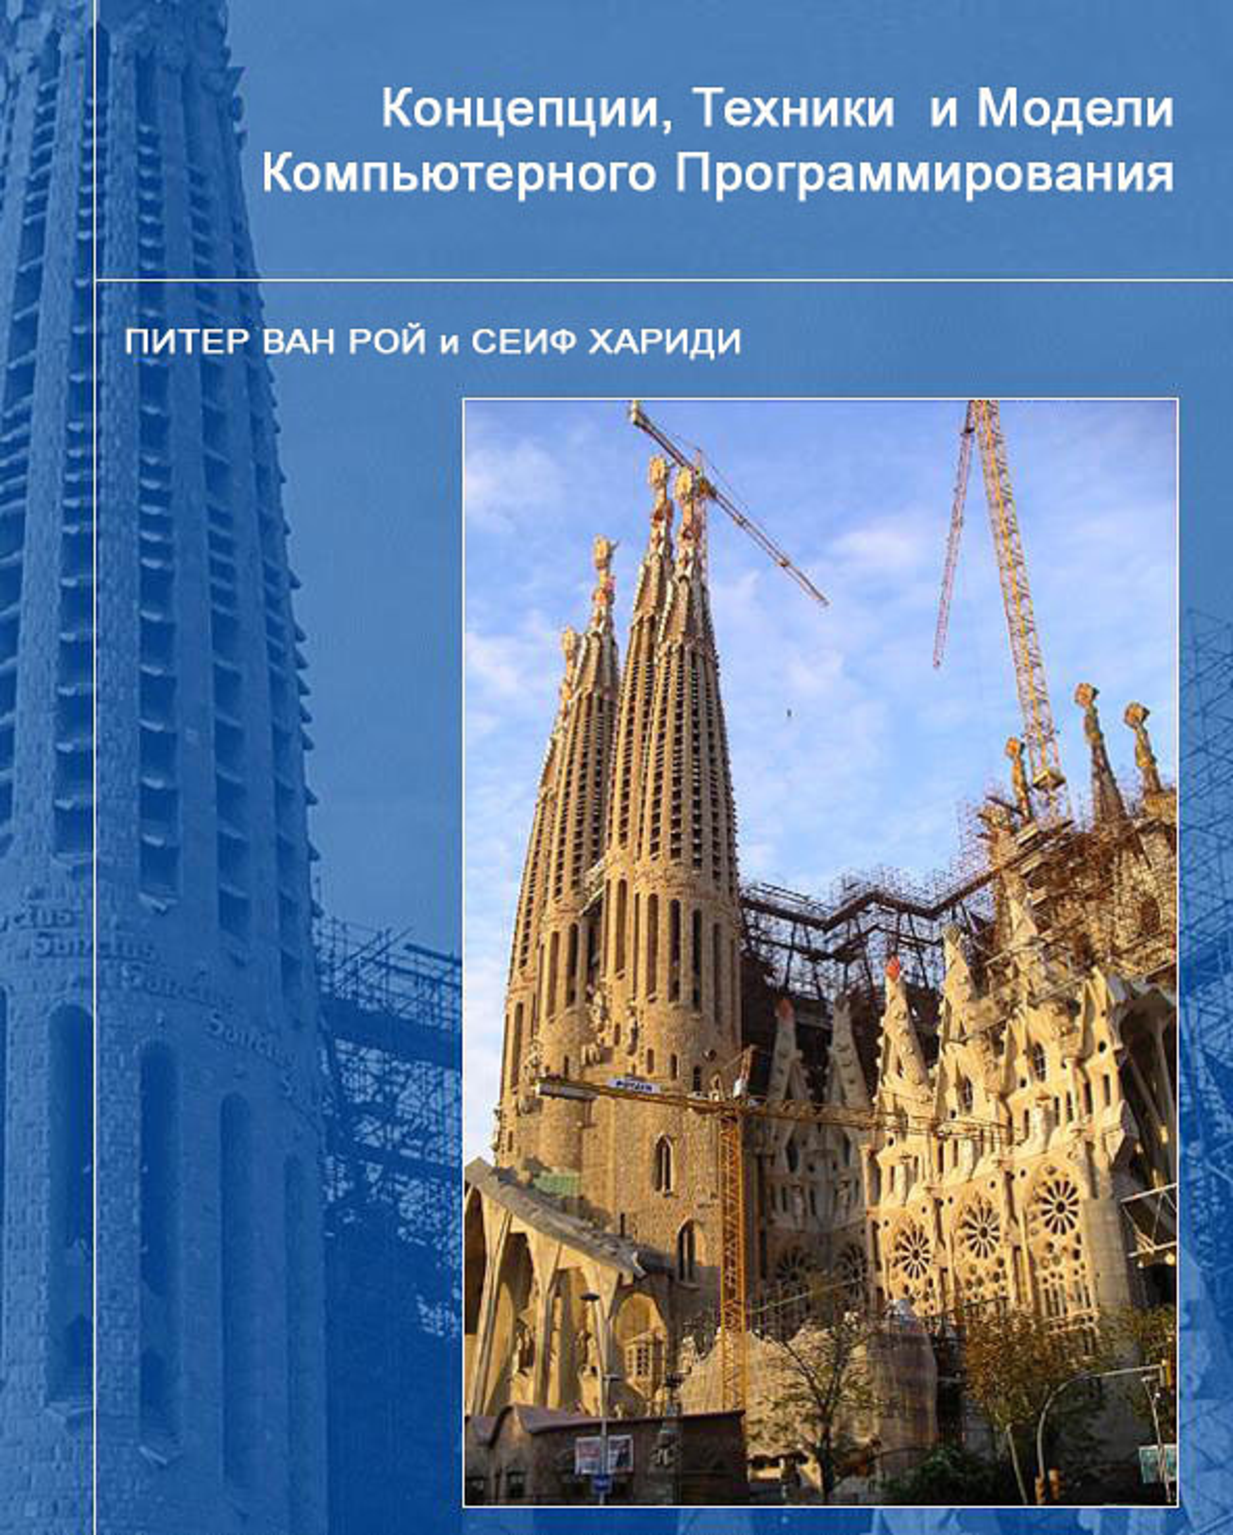
\includepdf{Cover.pdf}

{\let\newpage\relax\maketitle}
\maketitle
\tableofcontents
$$
\langle s \rangle \equiv \begin{cases}
  \text{\lstinline!local Max in!}\\
  \text{~~~~ \lstinline!local A in!}\\
  \text{~~~~~~~~ \lstinline!local B in!}\\
  \text{~~~~~~~~~~~~ \lstinline!local C in!}\\
  \langle s \rangle _1 \equiv \begin{cases}
    \text{~~~~~~~~\lstinline[mathescape=false]!Max=proc \{$ X Y Z\}!}\\
    \langle s \rangle _3 \equiv \begin{cases}
      \text{~~~~~~~~~~~~\lstinline!local T in!}\\
      \text{~~~~~~~~~~~~~~~~\lstinline!T=(X>=Y)!}\\
      \text{~~~~~~~~~} \langle s \rangle _4 \equiv \text{\lstinline!if T then Z=X else Z=Y end!}\\
      \text{~~~~~~~~~~\lstinline!end!}
    \end{cases}\\
    \text{~~~~~~~~~~~~\lstinline!end!}\\
    \text{~~~~~~~~\lstinline!A=3!}\\
    \text{~~~~~~~~\lstinline!B=5!}\\
    \langle s \rangle _2 \equiv \text{\lstinline!Max \{A B C\}!}\\
  \end{cases}\\
  \text{~~~~~~~~~~~~\lstinline!end!}\\
  \text{~~~~~~~~\lstinline!end!}\\
  \text{~~~~\lstinline!end!}\\
  \text{\lstinline!end!}
  \end{cases}
$$

\begin{lstlisting}
  fun {Fact N}
   if N =< 0 then 1 else N*{Fact N-1} end
end
 
fun {Comb N K}
   {Fact N} div ({Fact K} * {Fact N-K}) % integers can't overflow in Oz (unless no memory is left)
end
 
fun {SumList List}
   case List of nil then 0 $\frac{3}{4}$
   [] H|T then H+{SumList T} % pattern matching on lists
   end
end
\end{lstlisting}

kjdkasdjfksadjf ~~ dkjfsakjd dkjfkljds akdjfkdsj kkkk


\begin{thebibliography}{213}

\addcontentsline{toc}{chapter}{Литература}

\selectlanguage{english}
%\English

\bibitem{1}
Harold Abelson, Gerald Jay Sussman, and Julie Sussman. \emph{Structure and Interpretation of Computer Programs}. The MIT Press, Cambridge, Mass, 1985.

\bibitem{2}
Harold Abelson, Gerald Jay Sussman, and Julie Sussman. \emph{Structure and Interpretation of Computer Programs, Second Edition.} The MIT Press, Cambridge, Mass, 1996.

\bibitem{3}
Ili\`es Alouini and Peter Van Roy. Le protocole r\'eparti du langage Distributed Oz (The distributed protocol of the Distributed Oz language). In \emph{Colloque Francophone d’Ing\'enierie de Protocoles (CFIP 99)}, pages 283–298, April 1999.

\bibitem{4}
Edward G. Amoroso. \emph{Fundamentals of Computer Security Technology}. Prentice Hall, 1994.

\bibitem{5}
Ross J. Anderson. \emph{Security Engineering: A Guide to Building Dependable Distributed Systems.} John Wiley \& Sons, 2001.

\bibitem{6}
Gregory R. Andrews. \emph{Concurrent Programming: Principles and Practice}. Addison-Wesley, 1991.

\bibitem{7}
Joe Armstrong. Higher-order processes in Erlang, January 1997. Unpublished talk.

\bibitem{8}
Joe Armstrong. Concurrency oriented programming in Erlang, November 2002. Invited talk, Lightweight Languages Workshop 2002.

\bibitem{9}
Joe Armstrong, Mike Williams, Claes Wikstr\"om, and Robert Virding. \emph{Concurrent Programming in Erlang.} Prentice-Hall, Englewood Cliffs, N.J., 1996.

\bibitem{10}
Ken Arnold and James Gosling. \emph{The Java Programming Language, Second Edition.} Addison-Wesley, 1998.

\bibitem{11}
Arvind and R. E. Thomas. I-Structures: An efficient data type for functional languages. Technical Report 210, MIT, Laboratory for Computer Science, 1980.

\bibitem{12}
John Backus. Can programming be liberated from the von Neumann style? A functional style and its algebra of programs. \emph{Communications of the ACM}, 21(8):613–641, August 1978.

\bibitem{13}
John Backus. The history of FORTRAN I, II and III. \emph{ACM SIGPLAN Notices}, 13(8), August 1978.

\bibitem{14}
Henri E. Bal, Jennifer G. Steiner, and Andrew S. Tanenbaum. Programming languages for distributed computing systems. \emph{ACM Computing Surveys}, 21(3):261–322, September 1989.

\bibitem{15}
Holger B\"ar, Markus Bauer, Oliver Ciupke, Serge Demeyer, St\'ephane Ducasse, Michele Lanza, Radu Marinescu, Robb Nebbe, Oscar Nierstrasz, Michael Przybilski, Tamar Richner, Matthias Rieger, Claudio Riva, Anne-Marie Sassen, Benedikt Schulz, Patrick Steyaert, Sander Tichelaar, and Joachim Weisbrod. \emph{The FAMOOS Object-Oriented Reengineering Handbook.} October 1999. Result of ESPRIT project FAMOOS.

\bibitem{16}
Philip A. Bernstein, Vassos Hadzilacos, and Nathan Goodman. \emph{Concurrency Control and Recovery In Database Systems.} Addison-Wesley, 1987.

\bibitem{17}
Richard Bird. \emph{Introduction to Functional Programming using Haskell, Second Edition.} Prentice Hall, 1998.

\bibitem{18}
Andrew D. Birrell and Bruce Jay Nelson. Implementing remote procedure calls. \emph{ACM Transactions on Computer Systems}, 2(1):39–59, February 1984.

\bibitem{19}
Darius Blasband. Language engineering: from a hobby, to a research activity, to a trade, March 2002. Unpublished talk.

\bibitem{20}
Per Brand, Peter Van Roy, Rapha\"el Collet, and Erik Klintskog. Path redundancy in a mobile-state protocol as a primitive for language-based fault tolerance. Technical Report RR2000-01, D\'epartement d’Ing\'enierie Informatique, Universit\'e catholique de Louvain, 2000. Available at \verb"http://www.info.ucl.ac.be".

\bibitem{21}
Ivan Bratko. \emph{PROLOG Programming for Articial Intelligence, Third Edition}. Addison-Wesley, 2000.

\bibitem{22}
Per Brinch Hansen. Structured multiprogramming. \emph{Communications of the ACM}, 15(7):574–578, July 1972.

\bibitem{23}
Per Brinch Hansen. \emph{Operating System Principles}. Prentice Hall, 1973.

\bibitem{24}
Per Brinch Hansen. Java’s insecure parallelism. \emph{ACM SIGPLAN Notices}, 34(4):38–45, April 1999.

\bibitem{25}
Frederick P. Brooks, Jr. \emph{The Mythical Man-Month: Essays on Software Engineering}. Addison-Wesley, 1975.

\bibitem{26}
Frederick P. Brooks, Jr. \emph{The Mythical Man-Month: Essays on Software Engineering, Anniversary Edition}. Addison-Wesley, 1995.

\bibitem{27}
Timothy A. Budd. \emph{Multiparadigm Programming in Leda}. Addison-Wesley, 1995.

\bibitem{28}
Luca Cardelli. A language with distributed scope. In \emph{Principles of Programming Languages (POPL)}, pages 286–297, 1995.

\bibitem{29}
Mats Carlsson \emph{et al}. SICStus Prolog 3.8.1, December 1999. Available at \verb"http://www.sics.se".

\bibitem{30}
Nicholas Carriero and David Gelernter. Linda in context. \emph{Communications of the ACM}, 32(4):444–458, 1989.

\bibitem{31}
Nicholas Carriero and David Gelernter. Coordination languages and their significance. \emph{Communications of the ACM}, 35(2):96–107, February 1992.

\bibitem{32}
Emmanuel Chailloux, Pascal Manoury, and Bruno Pagano. \emph{D\'eveloppement d’applications avec Objective Caml}. O’Reilly, Paris, France, 2000.

\bibitem{33}
Randy Chow and Theodore Johnson. \emph{Distributed Operating Systems and Algorithms}. Addison-Wesley, San Francisco, Calif., 1997.

\bibitem{34}
Keith L. Clark. PARLOG: the language and its applications. In A. J. Nijman J. W. de Bakker and P. C. Treleaven, editors, \emph{Proceedings of the Conference on Parallel Architectures and Languages Europe (PARLE). Volume II: Parallel Languages, volume 259 of Lecture Notes in Computer Science}, pages 30–53, Eindhoven, The Netherlands, June 1987. Springer.

\bibitem{35}
Keith L. Clark and Frank McCabe. The control facilities of IC-Prolog. In D. Michie, editor, \emph{Expert Systems in the Micro-Electronic Age}, pages 122–149. Edinburgh University Press, Edinburgh, Scotland, 1979.

\bibitem{36}
Keith L. Clark, Frank G. McCabe, and Steve Gregory. IC-PROLOG — language features. In Keith L. Clark and Sten-\r{A}ke T\"arnlund, editors, \emph{Logic Programming}, pages 253–266. Academic Press, London, 1982.

\bibitem{37}
Arthur C. Clarke. \emph{Profiles of the Future}. Pan Books, 1973. Revised edition.

\bibitem{38}
William Clinger and Jonathan Rees. The revised report on the algorithmic language Scheme. \emph{LISP Pointers}, IV(3):1–55, July-September 1991.

\bibitem{39}
Helder Coelho and Jos\'e C. Cotta. \emph{Prolog by Example: How to Learn, Teach, and Use It}. Springer-Verlag, 1988.

\bibitem{40}
Alain Colmerauer. The birth of Prolog. In \emph{The Second ACM-SIGPLAN History of Programming Languages Conference}, pages 37–52, March 1993. ACM SIGPLAN Notices.

\bibitem{41}
Thomas H. Cormen, Charles E. Leiserson, and Ronald L. Rivest. \emph{Introduction to Algorithms}. The MIT Press, McGraw-Hill, 1990.

\bibitem{42}
C. J. Date. \emph{An Introduction to Database Systems}. Addison-Wesley, 1994.

\bibitem{43}
Harvey M. Deitel. \emph{An Introduction to Operating Systems}. Addison-Wesley, 1984.

\bibitem{44}
Serge Demeyer, St\'ephane Ducasse, Oscar Nierstrasz, and Ralph E. Johnson. \emph{Object Oriented Reengineering Patterns}. Morgan Kaufmann, 2002.

\bibitem{45}
Edsger W. Dijkstra. \emph{A Primer of Algol 60 Programming}. Academic Press, 1962.

\bibitem{46}
Edsger W. Dijkstra. Go To statement considered harmful. \emph{Communications of the ACM}, 11(3):147–148, March 1968.

\bibitem{47}
Denys Duchier. Loop support. Technical report, DFKI and Saarland University, December 2001. Available at \verb"http://www.mozart-oz.org/".

\bibitem{48}
Denys Duchier, Claire Gardent, and Joachim Niehren. Concurrent constraint programming in Oz for natural language processing. Technical report, Saarland University, Saarbr\"ucken, Germany, 1999. Available at \verb"http://www.ps.uni-sb.de/Papers/abstracts/oznlp.html".

\bibitem{49}
Denys Duchier, Leif Kornstaedt, and Christian Schulte. The Oz base environment. Technical report, Mozart Consortium, December 2001. Available at \verb"http://www.mozart-oz.org/".

\bibitem{50}
Denys Duchier, Leif Kornstaedt, Christian Schulte, and Gert Smolka. A Higher-order Module Discipline with Separate Compilation, Dynamic Linking, and Pickling. Technical report, Programming Systems Lab, DFKI and Saarland University, 1998. DRAFT. Available at \verb"http://www.mozart-oz.org/papers/".

\bibitem{51}
R. Kent Dybvig, Carl Bruggeman, and David Eby. generation-based garbage collector, June 1993.

\bibitem{52}
E. W. Elcock. Absys: The first logic programming language–a retrospective and a commentary. \emph{Journal of Logic Programming}, 9(1):1–17, 1990.

\bibitem{53}
Robert W. Floyd. Nondeterministic algorithms. \emph{Journal of the ACM}, 14(4):636–644, October 1967.

\bibitem{54}
Martin Fowler and Kendall Scott. \emph{UML Distilled: A Brief Guide to the Standard Object Modeling Language}. Addison-Wesley Longman, Inc., 2000.

\bibitem{55}
Michael J. French. \emph{Invention and evolution: design in nature and engineering}. Cambridge University Press, 1988.

\bibitem{56}
Daniel P. Friedman, Mitchell Wand, and Christopher T. Haynes. \emph{Essentials of Programming Languages}. The MIT Press, 1992.

\bibitem{57}
Tetsuro Fujise, Takashi Chikayama, Kazuaki Rokusawa, and Akihiko Nakase. KLIC: A portable implementation of KL1. In \emph{Fifth Generation Computing Systems (FGCS ’94)}, pages 66–79, December 1994.

\bibitem{58}
Erich Gamma, Richard Helm, Ralph Johnson, and John Vlissides. \emph{Design Patterns: Elements of Reusable Object-Oriented Software}. Addison-Wesley, 1994.

\bibitem{59}
David Gelernter. Generative communication in Linda. \emph{ACM Transactions on Programming Languages and Systems}, 7(1):80–112, January 1985.

\bibitem{60}
Adele Goldberg and David Robson. \emph{Smalltalk-80: The language and its implementation}. Addison-Wesley, 1983.

\bibitem{61}
Danny Goodman. \emph{Dynamic HTML: The Definitive Reference, Second Edition}. O’Reilly \& Associates, 2002.

\bibitem{62}
James Edward Gordon. \emph{The Science of Structures and Materials}. Scientific American Library, 1988.

\bibitem{63}
James Gosling, Bill Joy, and Guy Steele. \emph{The Java Language Specification}. Addison-Wesley, 1996. Available at http://www.javasoft.com.

\bibitem{64}
Jim Gray and Andreas Reuter. \emph{Transaction Processing – Concepts and Techniques}. Morgan Kaufmann, 1993.

\bibitem{65}
Donatien Grolaux. QTk module, 2000. Available \verb"http://www.mozart-oz.org/mozart-stdlib/index.html".

\bibitem{66}
Donatien Grolaux, Peter Van Roy, and Jean Vanderdonckt. QTk – a mixed declarative/procedural approach for designing executable user interfaces. In \emph{8th IFIP Working Conference on Engineering for Human-Computer Interaction (EHCI’01)}, Lecture Notes in Computer Science, Toronto, Canada, May 2001. Springer-Verlag. Short paper.

\bibitem{67}
Donatien Grolaux, Peter Van Roy, and Jean Vanderdonckt. QTk – an integrated model-based approach to designing executable user interfaces. In \emph{8th Workshop on Design, Specification, and Verification of Interactive Systems (DSVIS 2001)}, Lecture Notes in Computer Science, Glasgow, Scotland, June 2001. Springer-Verlag.

\bibitem{68}
Robert H. Halstead, Jr. MultiLisp: A language for concurrent symbolic computation. \emph{ACM Transactions on Programming Languages and Systems}, 7(4):501–538, October 1985.

\bibitem{69}
Richard Hamming. \emph{The Art of Doing SCIENCE and Engineering: Learning to Learn}. Gordon and Breach Science Publishers, 1997.

\bibitem{70}
Seif Haridi and Sverker Janson. Kernel Andorra Prolog and its computation model. In \emph{7th International Conference on Logic Programming}, pages 31–48. The MIT Press, June 1990.

\bibitem{71}
Seif Haridi, Peter Van Roy, Per Brand, Michael Mehl, Ralf Scheidhauer, and Gert Smolka. Efficient logic variables for distributed computing. \emph{ACM Transactions on Programming Languages and Systems}, May 1999.

\bibitem{72}
Seif Haridi, Peter Van Roy, Per Brand, and Christian Schulte. Programming languages for distributed applications. \emph{New Generation Computing}, 16(3):223–261, May 1998.

\bibitem{73}
Seif Haridi, Peter Van Roy, and Gert Smolka. An overview of the design of Distributed Oz. In the \emph{2nd International Symposium on Parallel Symbolic Computation (PASCO 97)}. ACM, July 1997.

\bibitem{74}
Martin Henz. \emph{Objects for Concurrent Constraint Programming}. Internationale Series in Engineering and Computer Science. Kluwer Academic Publishers, Boston, MA, USA, 1997.

\bibitem{75}
Martin Henz. \emph{Objects for Concurrent Constraint Programming}, volume 426 of \emph{The Kluwer International Series in Engineering and Computer Science}. Kluwer Academic Publishers, Boston, November 1997.

\bibitem{76}
Martin Henz. Objects in Oz. Doctoral dissertation, Saarland University, Saarbr\"ucken, Germany, May 1997.

\bibitem{77}
Martin Henz and Leif Kornstaedt. The Oz notation. Technical report, DFKI and Saarland University, December 1999. Available at \verb"http://www.mozart-oz.org/".

\bibitem{78}
Martin Henz, Tobias M\"uller, and Ka Boon Ng. Figaro: Yet another constraint programming library. In \emph{Workshop on Parallelism and Implementation Technology for Constraint Logic Programming, International Conference on Logic Programming (ICLP 99)}, 1999.

\bibitem{79}
Martin Henz, Gert Smolka, and J\"org W\"urtz. Oz – a programming language for multi-agent systems. In \emph{13th International Joint Conference on Artificial Intelligence}, pages 404–409. Morgan Kaufmann, August 1993.

\bibitem{80}
Martin Henz, Gert Smolka, and J\"org W\"urtz. Oz—a programming language for multi-agent systems. In Ruzena Bajcsy, editor, \emph{13th International Joint Conference on Artificial Intelligence}, volume 1, pages 404–409, Chamb\'ery, France, 30 August–3 September 1993. Morgan Kaufmann Publishers.

\bibitem{81}
Martin Henz, Gert Smolka, and J\"org W\"urtz. Object-oriented concurrent constraint programming in Oz. In Pascal Van Hentenryck and Vijay Saraswat, editors, \emph{Principles and Practice of Constraint Programming}, pages 29–48, Cambridge, Mass., 1995. The MIT Press.

\bibitem{82}
Charles Antony Richard Hoare. Monitors: An operating system structuring concept. \emph{Communications of the ACM}, 17(10):549–557, October 1974.

\bibitem{83}
Charles Antony Richard Hoare. Communicating sequential processes. \emph{Communications of the ACM}, 21(8):666–677, August 1978.

\bibitem{84}
Bruce K. Holmer, Barton Sano, Michael Carlton, Peter Van Roy, and Alvin M. Despain. Design and analysis of hardware for high performance Prolog. \emph{J. Log. Prog.}, 29:107–139, November 1996.

\bibitem{85}
Paul Hudak. Conception, evolution, and application of functional programming languages. \emph{Computing Surveys}, 21(3):359–411, September 1989.

\bibitem{86}
Paul Hudak, John Peterson, and Joseph Fasel. A gentle introduction to Haskell version 98. Available at \verb"http://www.haskell.org/tutorial/".

\bibitem{87}
John Hughes. Why Functional Programming Matters. \emph{Computer Journal}, 32(2):98–107, 1989.

\bibitem{88}
Robert A. Iannucci. Parallel Machines: \emph{Parallel Machine Languages. The Emergence of Hybrid Dataflow Computer Architectures}. Kluwer, Dordrecht, the Netherlands, 1990.

\bibitem{89}
Daniel H. H. Ingalls. Design principles behind Smalltalk. \emph{Byte}, 6(8):286–298, 1981.

\bibitem{90}
Joxan Jaffar and Michael Maher. Constraint logic programming: A survey. \emph{J. Log. Prog.}, 19/20:503–581, May/July 1994.

\bibitem{91}
Raj Jain. \emph{The Art of Computer Systems Performance Analysis}. Wiley Professional Computing, 1991.

\bibitem{92}
Sverker Janson. \emph{AKL–A Multiparadigm Programming Language}. PhD thesis, Uppsala University and SICS, 1994.

\bibitem{93}
Sverker Janson and Seif Haridi. Programming paradigms of the Andorra Kernel Language. In \emph{International Symposium on Logic Programming}, pages 167–183, October 1991.

\bibitem{94}
K. Jensen and N. Wirth. \emph{Pascal: User Manual and Report (Second Edition)}. Springer-Verlag, 1978.

\bibitem{95}
Richard Jones and Rafael Lins. \emph{Garbage Collection: Algorithms for Automatic Dynamic Memory Management}. John Wiley \& Sons, 1996.

\bibitem{96}
Andreas K\r{a}gedal, Peter Van Roy, and Bruno Dumant. Logical State Threads 0.1, January 1997. Available at http://www.info.ucl.ac.be/people/PVR/implementation.html.

\bibitem{97}
Gilles Kahn. The semantics of a simple language for parallel programming. In \emph{IFIP Congress}, pages 471–475, 1974.

\bibitem{98}
Gilles Kahn and David B. MacQueen. Coroutines and networks of parallel processes. In \emph{IFIP Congress}, pages 993–998, 1977.

\bibitem{99}
B. W. Kernighan and D. M. Ritchie. \emph{The C Programming Language (ANSI C), Second Edition}. Prentice Hall, 1988.

\bibitem{100}
Gregor Kiczales, Jim des Rivi\`eres, and Daniel G. Bobrow. \emph{The Art of the Metaobject Protocol}. The MIT Press, 1991.

\bibitem{101}
Donald E. Knuth. \emph{The Art of Computer Programming: Seminumerical Algorithms}, volume 2. Addison-Wesley.

\bibitem{102}
Donald E. Knuth. \emph{The Art of Computer Programming: Fundamental Algorithms}, volume 1. Addison-Wesley, 1973.

\bibitem{103}
Donald E. Knuth. Structured programming with \textbf{go to} statements. \emph{Computing Surveys}, 6(4), December 1974.

\bibitem{104}
Leif Kornstaedt. Gump – a front-end generator for Oz. Technical report, Mozart Consortium, December 2001. Available at \verb"http://www.mozart-oz.org/".

\bibitem{105}
S. Rao Kosaraju. Analysis of structured programs. \emph{J. Computer and System Sciences}, 9(3), December 1974.

\bibitem{106}
Robert Kowalski. \emph{Logic for Problem Solving}. North-Holland, 1979.

\bibitem{107}
James F. Kurose and Keith W. Ross. \emph{Computer networking: a top-down approach featuring the Internet}. Addison-Wesley, 2001.

\bibitem{108}
Leslie Lamport. \emph{\LaTeX: A Document Preparation System, Second Edition}. Addison-Wesley, 1994.

\bibitem{109}
Hugh C. Lauer and Roger M. Needham. On the duality of operating system structures. In \emph{Second International Symposium on Operating Systems, IRIA}, October 1978. Reprinted in \emph{Operating Systems Review}, 13(2), April 1979, pp. 3–19.

\bibitem{110}
Doug Lea. \emph{Concurrent Programming in Java}. Addison-Wesley, 1997.

\bibitem{111}
Doug Lea. \emph{Concurrent Programming in Java, Second Edition}. Addison-Wesley, 2000.

\bibitem{112}
Nancy Leveson and Clark S. Turner. An investigation of the Therac-25 accidents. \emph{IEEE Computer}, 26(7):18–41, July 1993.

\bibitem{113}
Henry Lieberman. Using prototypical objects to implement shared behavior in object-oriented systems. In \emph{1st Conference on Object-Oriented Programming Languages, Systems, and Applications (OOPSLA 86)}, September 1986. Also in Object-Oriented Computing, Gerald Peterson, ed., IEEE Computer Society Press, 1987.

\bibitem{114}
John Lloyd. \emph{Foundations of Logic Programming, Second Edition}. Springer-Verlag, 1987.

\bibitem{115}
Nancy Lynch. \emph{Distributed Algorithms}. Morgan Kaufmann, San Francisco, Calif., 1996.

\bibitem{116}
Bruce J. MacLennan. \emph{Principles of Programming Languages, Second Edition}. Saunders, Harcourt Brace Jovanovich, 1987.

\bibitem{117}
Michael Maher. Logic semantics for a class of committed-choice programs. In \emph{International Conference on Logic Programming (ICLP 87)}, pages 858–876, May 1987.

\bibitem{118}
Zohar Manna. \emph{The Mathematical Theory of Computation}. McGraw-Hill, 1974.

\bibitem{119}
Sun Microsystems. \emph{The Remote Method Invocation Specification}, 1997. Available at http://www.javasoft.com.

\bibitem{120}
John McCarthy. \emph{LISP 1.5 Programmer’s Manual}. The MIT Press, 1962.

\bibitem{121}
Michael Mehl, Christian Schulte, and Gert Smolka. Futures and by-need synchronization for Oz. DRAFT. Available at \verb"http://www.mozart-oz.org/papers/", May 1998.

\bibitem{122}
Bertrand Meyer. \emph{Object-Oriented Software Construction, Second Edition}. Prentice Hall, 2000.

\bibitem{123}
Mark Miller, Marc Stiegler, Tyler Close, Bill Frantz, Ka-Ping Yee, Chip Morningstar, Jonathan Shapiro, and Norm Hardy. E: Open source distributed capabilities, 2001. Available at \verb"http://www.erights.org".

\bibitem{124}
Mark Miller, Ka-Ping Yee, and Jonathan Shapiro. Capability myths demolished. Draft available at \verb"http://zesty.ca/capmyths", 2003.

\bibitem{125}
Mark S. Miller, Chip Morningstar, and Bill Frantz. Capability-based financial instruments. In \emph{Financial Cryptography 2000}, Anguilla, British West Indies, February 2000.

\bibitem{126}
Robin Milner, Mads Tofte, and Robert Harper. \emph{Definition of Standard ML}. MIT Press, Cambridge, MA, USA, 1990.

\bibitem{127}
J. Paul Morrison. \emph{Flow-Based Programming: A New Approach to Application Development}. Van Nostrand Reinhold, 1994.

\bibitem{128}
Almetwally Mostafa, Ili\`es Alouini, and Peter Van Roy. Fault tolerant global store module, 2001. Available at \verb"http://www.mozart-oz.org/mogul/info/mostafa/globalstore.html".

\bibitem{129}
Mozart Consortium. The Mozart Programming System version 1.2.3, December 2001. Available at \verb"http://www.mozart-oz.org/".

\bibitem{130}
Peter Naur. Revised report on the algorithmic language ALGOL 60. \emph{Communications of the ACM}, 1963.

\bibitem{131}
Rishiyur S. Nikhil. ID language reference manual version 90.1. Technical Report Memo 284-2, MIT, Computation Structures Group, July 1994.

\bibitem{132}
Rishiyur S. Nikhil. An overview of the parallel language Id – a foundation for pH, a parallel dialect of Haskell. Technical report, Digital Equipment Corporation, Cambridge Research Laboratory, 1994.

\bibitem{133}
Rishiyur S. Nikhil and Arvind. \emph{Implicit Parallel Programming in pH}. Morgan Kaufmann, 2001.

\bibitem{134}
Donald A. Norman. \emph{The Design of Everyday Things}. Basic Books, Inc., 1988.

\bibitem{135}
Theodore Norvell. Monads for the working Haskell programmer – a short tutorial. Available at \verb"http://www.haskell.org/".

\bibitem{136}
Peter Norvig. \emph{Paradigms of Artificial Intelligence Programming: Case Studies in Common Lisp}. Morgan Kaufmann, 1992.

\bibitem{137}
K. Nygaard and O. J. Dahl. \emph{The Development of the SIMULA Languages}, pages 439–493. Academic Press, 1981.

\bibitem{138}
Chris Okasaki. \emph{Purely Functional Data Structures}. Cambridge University Press, 1998.

\bibitem{139}
Richard A. O’Keefe. \emph{The Craft of Prolog}. The MIT Press, 1990.

\bibitem{140}
Andreas Paepcke, editor. \emph{Object-Oriented Programming: The CLOS Perspective}. The MIT Press, 1993.

\bibitem{141}
Seymour Papert. \emph{Mindstorms: Children, Computers, and Powerful Ideas}. The Harvester Press, 1980.

\bibitem{142}
David Lorge Parnas. On the criteria to be used in decomposing systems into modules. \emph{Communications of the ACM}, 15(12):1053–1058, December 1972.

\bibitem{143}
David Lorge Parnas. Teaching programming as engineering. In \emph{9th International Conference of Z Users}, volume 967 of \emph{Lecture Notes in Computer Science}. Springer-Verlag, 1995. Reprinted in \emph{Software Fundamentals}, Addison-Wesley, 2001.

\bibitem{144}
David Lorge Parnas. \emph{Software Fundamentals}. Addison-Wesley, 2001.

\bibitem{145}
F. Patern\`o. \emph{Model-based Design and Evaluation of Interactive Applications}. Springer-Verlag, Berlin, 1999.

\bibitem{146}
David A. Patterson and John L. Hennessy. \emph{Computer Architecture: A Quantitative Approach, Second Edition}. Morgan Kaufmann, 1996.

\bibitem{147}
Simon Peyton Jones. Tackling the awkward squad: monadic input/output, concurrency, exceptions, and foreign-language calls in Haskell. In Tony Hoare, Manfred Broy, and Ralf Steinbruggen, editors, \emph{Engineering theories of software construction}, pages 47–96. IOS Press, 2001. Presented at the 2000 Marktoberdorf Summer School.

\bibitem{148}
Simon Peyton Jones, editor. \emph{Haskell 98 language and libraries: The revised report}. Cambridge University Press, 2003. Also published as the January 2003 Special Issue of the Journal of Functional Programming.

\bibitem{149}
Simon Peyton Jones, Andrew Gordon, and Sigbjorn Finne. Concurrent Haskell. In \emph{Principles of Programming Languages (POPL)}, 1996.

\bibitem{150}
Shari Lawrence Pfleeger. \emph{Software Engineering: The Production of Quality Software, Second Edition}. Macmillan, 1991.

\bibitem{151}
David Plainfoss\'e and Marc Shapiro. A survey of distributed garbage collection techniques. In the \emph{International Workshop on Memory Management}, volume 986 of \emph{Lecture Notes in Computer Science}, pages 211–249, Berlin, September 1995. Springer-Verlag.

\bibitem{152}
R. J. Pooley. \emph{An Introduction to Programming in SIMULA}. Blackwell Scientific Publishers, 1987.

\bibitem{153}
William H. Press, Brian P. Flannery, Saul A. Teukolsky, and William T. Vetterling. \emph{Numerical Recipes: The Art of Scientific Computing}. Cambridge University Press, 1986.

\bibitem{154}
Roger S. Pressman. \emph{Software Engineering, Sixth Edition}. Addison-Wesley, 2000.

\bibitem{155}
Mahmoud Rafea, Fredrik Holmgren, Konstantin Popov, Seif Haridi, Stelios Lelis, Petros Kavassalis, and Jakka Sairamesh. Application architecture of the Internet simulation model: Web Word of Mouth (WoM). In \emph{IASTED International Conference on Modelling and Simulation MS2002}, May 2002.

\bibitem{156}
Eric Raymond. The cathedral and the bazaar, May 1997.

\bibitem{157}
Juris Reinfelds. Teaching of programming with a programmer’s theory of programming. In \emph{Informatics Curricula, Teaching Methods, and Best Practice (ICTEM 2002, IFIP Working Group 3.2 Working Conference)}. Kluwer Academic Publishers, 2002.

\bibitem{158}
John H. Reppy. \emph{Concurrent Programming in ML}. Cambridge University Press, 1999.

\bibitem{159}
James Rumbaugh, Ivar Jacobson, and Grady Booch. \emph{The Unified Modeling Language reference manual}. Addison-Wesley, 1999.

\bibitem{160}
Stuart Russell and Peter Norvig. \emph{Artificial Intelligence: A modern approach}. Prentice Hall, 1995.

\bibitem{161}
Oliver Sacks. \emph{The Man Who Mistook His Wife for a Hat: And Other Clinical Tales}. Touchstone Books, 1998.

\bibitem{162}
Jakka Sairamesh, Petros Kavassalis, Manolis Marazakis, Christos Nikolaos, and Seif Haridi. Information cities over the Internet: Taxonomy, principles and architecture. In \emph{Digital Communities 2002}, November 2001.

\bibitem{163}
Vijay A. Saraswat. \emph{Concurrent Constraint Programming}. The MIT Press, 1993.

\bibitem{164}
Vijay A. Saraswat, Martin C. Rinard, and Prakash Panangaden. Semantic foundations of concurrent constraint programming. In \emph{Principles of Programming Languages (POPL)}, pages 333–352, 1991.

\bibitem{165}
Steve Schneider. \emph{Concurrent and Real-time Systems: The CSP Approach}. John Wiley \& Sons, 2000.

\bibitem{166}
Bruce Schneier. \emph{Applied Cryptography}. John Wiley \& Sons, 1996.

\bibitem{167}
Christian Schulte. Programming constraint inference engines. In Gert Smolka, editor, \emph{Proceedings of the Third International Conference on Principles and Practice of Constraint Programming}, volume 1330 of \emph{Lecture Notes in Computer Science}, pages 519–533, Schloß Hagenberg, Austria, October 1997. Springer-Verlag.

\bibitem{168}
Christian Schulte. Comparing trailing and copying for constraint programming. In \emph{International Conference on Logic Programming (ICLP 99)}, pages 275–289. The MIT Press, November 1999.

\bibitem{169}
Christian Schulte. \emph{Programming Constraint Inference Services}. PhD thesis, Saarland University, Fachbereich Informatik, Saarbr\"ucken, Germany, 2000.

\bibitem{170}
Christian Schulte. Programming deep concurrent constraint combinators. In Enrico Pontelli and V\'\i tor Santos Costa, editors, \emph{Practical Aspects of Declarative Languages, Second International Workshop, PADL 2000}, volume 1753 of \emph{Lecture Notes in Computer Science}, pages 215–229, Boston, MA, USA, January 2000. Springer-Verlag.

\bibitem{171}
Christian Schulte. Oz Explorer – visual constraint programming support. Technical report, Mozart Consortium, December 2001. Available at \verb"http://www.mozart-oz.org/".

\bibitem{172}
Christian Schulte. \emph{Programming Constraint Services: High-Level Programming of Standard and New Constraint Services}, volume 2302 of \emph{Lecture Notes in Computer Science}. Springer-Verlag, 2002.

\bibitem{173}
Christian Schulte and Gert Smolka. Encapsulated search for higher-order concurrent constraint programming. In \emph{1994 International Symposium on Logic Programming}, pages 505–520. The MIT Press, November 1994.

\bibitem{174}
Christian Schulte and Gert Smolka. Finite domain constraint programming in Oz. A tutorial. Technical report, DFKI and Saarland University, December 1999. Available at \verb"http://www.mozart-oz.org/".

\bibitem{175}
Ehud Shapiro. A subset of Concurrent Prolog and its interpreter. Technical Report TR-003, Institute for New Generation Computer Technology (ICOT), Cambridge, Mass., January 1983.

\bibitem{176}
Ehud Shapiro, editor. \emph{Concurrent Prolog: Collected Papers}, volume 1-2. The MIT Press, Cambridge, Mass., 1987.

\bibitem{177}
Ehud Shapiro. The family of concurrent logic programming languages. \emph{ACM Computing Surveys}, 21(3):413–510, September 1989.

\bibitem{178}
Daniel P. Siewiorek, C. Gordon Bell, and Allen Newell. \emph{Computer Structures: Principles and Examples}. McGraw-Hill Book Company, 1982.

\bibitem{179}
Gert Smolka. The definition of Kernel Oz. In Andreas Podelski, editor, \emph{Constraints: Basics and Trends}, volume 910 of \emph{Lecture Notes in Computer Science}, pages 251–292. Springer-Verlag, Berlin, 1995.

\bibitem{180}
Gert Smolka. The Oz programming model. In \emph{Computer Science Today}, volume 1000 of \emph{Lecture Notes in Computer Science}, pages 324–343. Springer-Verlag, Berlin, 1995.

\bibitem{181}
Guy L. Steele, Jr. \emph{Common LISP: The Language}. Digital Press, 1984.

\bibitem{182}
Leon Sterling and Ehud Shapiro. \emph{The Art of Prolog–Advanced Programming Techniques}. Series in Logic Programming. The MIT Press, 1986.

\bibitem{183}
Marc Stiegler. \emph{The E Language in a Walnut}. 2000. Draft, available at \verb"http://www.erights.org".

\bibitem{184}
Bjarne Stroustrup. \emph{The C++ Programming Language, Third Edition}. Addison-Wesley, 1997.

\bibitem{185}
Giancarlo Succi and Michele Marchesi. \emph{Extreme Programming Examined}. Addison-Wesley, 2001.

\bibitem{186}
Sun Microsystems. \emph{The Java Series}. Sun Microsystems, Mountain View, Calif., 1996. Available at http://www.javasoft.com.

\bibitem{187}
Clemens Szyperski. \emph{Component Software: Beyond Object-Oriented Programming}. Addison-Wesley and ACM Press, 1999.

\bibitem{188}
Andrew Taylor. \emph{High-Performance Prolog Implementation}. PhD thesis, Basser Department of Computer Science, University of Sydney, June 1991.

\bibitem{189}
Gerard Tel. \emph{An Introduction to Distributed Algorithms}. Cambridge University Press, Cambridge, United Kingdom, 1994.

\bibitem{190}
Evan Tick. The deevolution of concurrent logic programming. \emph{J. Log. Prog.}, 23(2):89–123, May 1995.

\bibitem{191}
Kasunori Ueda. Guarded Horn Clauses. In Eiti Wada, editor, \emph{Proceedings of the 4th Conference on Logic Programming}, volume 221 of \emph{Lecture Notes in Computer Science}, pages 168–179, Tokyo, Japan, July 1985. Springer.

\bibitem{192}
Jeffrey D. Ullman. \emph{Elements of ML Programming}. Prentice Hall, 1998.

\bibitem{193}
Peter Van Roy. VLSI-BAM Diagnostic Generator, 1989. Prolog program to generate assembly language diagnostics. Aquarius Project, University of California, Berkeley.

\bibitem{194}
Peter Van Roy. \emph{Can Logic Programming Execute as Fast as Imperative Programming?} PhD thesis, Computer Science Division, University of California at Berkeley, December 1990. Technical Report UCB/CSD 90/600.

\bibitem{195}
Peter Van Roy. 1983–1993: The wonder years of sequential Prolog implementation. \emph{J. Log. Prog.}, 19/20:385–441, May/July 1994.

\bibitem{196}
Peter Van Roy, Per Brand, Denys Duchier, Seif Haridi, Martin Henz, and Christian Schulte. Logic programming in the context of multiparadigm programming: the Oz experience. \emph{Theory and Practice of Logic Programming}, 2003. To appear.

\bibitem{197}
Peter Van Roy, Per Brand, Seif Haridi, and Rapha\"el Collet. A lightweight reliable object migration protocol. In Henri E. Bal, Boumediene Belkhouche, and Luca Cardelli, editors, \emph{Internet Programming Languages,} volume 1686 of \emph{Lecture Notes in Computer Science}. Springer Verlag, October 1999.

\bibitem{198}
Peter Van Roy and Alvin Despain. High-performance logic programming with the Aquarius Prolog compiler. \emph{IEEE Computer,} pages 54–68, January 1992.

\bibitem{199}
Peter Van Roy and Seif Haridi. Teaching programming broadly and deeply: the kernel language approach. In \emph{Informatics Curricula, Teaching Methods, and Best Practice (ICTEM 2002, IFIP Working Group 3.2 Working Conference)}. Kluwer Academic Publishers, 2002.

\bibitem{200}
Peter Van Roy and Seif Haridi. Teaching programming with the kernel language approach. In \emph{Workshop on Functional and Declarative Programming in Education (FDPE02), at Principles, Logics, and Implementations of High-Level Programming Languages (PLI2002)}. University of Kiel, Germany, October 2002.

\bibitem{201}
Peter Van Roy, Seif Haridi, Per Brand, Gert Smolka, Michael Mehl, and Ralf Scheidhauer. Mobile objects in Distributed Oz. \emph{ACM Transactions on Programming Languages and Systems,} 19(5):804–851, September 1997.

\bibitem{202}
Arthur H. Veen. Dataflow machine architecture. \emph{ACM Computing Surveys,} 18(4):365–396, December 1986.

\bibitem{203}
Duncan J. Watts. \emph{Small Worlds: The Dynamics of Networks between Order and Randomness.} Princeton University Press, 1999.

\bibitem{204}
Gerhard Weikum and Gottfried Vossen. \emph{Transactional Information Systems: Theory, Algorithms, and the Practice of Concurrency Control and Recovery.} Morgan Kaufmann, 2002.

\bibitem{205}
Gerhard Weiss, editor. \emph{Multiagent Systems: A Modern Approach to Distributed Artificial Intelligence.} The MIT Press, 1999.

\bibitem{206}
Claes Wikstr\"om. Distributed programming in Erlang. In the \emph{1st International Symposium on Parallel Symbolic Computation (PASCO 94 ),} pages 412–421, Singapore, September 1994. World Scientific.

\bibitem{207}
Herbert S. Wilf. \emph{generatingfunctionology.} Academic Press, 1994.

\bibitem{208}
Glynn Winskel. \emph{The Formal Semantics of Programming Languages.} Foundations of Computing Series. The MIT Press, Cambridge, Massachusetts, 1993.

\bibitem{209}
Noel Winstanley. What the hell are Monads?, 1999. Available at \verb"http://www.haskell.org".

\bibitem{210}
David Wood. Use of objects and agents at Symbian, September 2000. Talk given at the Newcastle Seminar on the Teaching of Computing Science.

\bibitem{211}
Matthias Zenger and Martin Odersky. Implementing extensible compilers. In \emph{1st International Workshop on Multiparadigm Programming with Object-Oriented Languages,} pages 61–80. John von Neumann Institute for Computing (NIC), June 2001. Workshop held as part of ECOOP 2001.

\end{thebibliography}

\end{document}
